\subsection*{Problema 25}

\textbf{Enunciado:} Calcular la integral:
\begin{equation*}
\int \dfrac{x^2 + 2x + 3}{x^3 - x} \, dx
\end{equation*}

\textbf{Solución:} 

Primero, factorizamos el denominador de la función racional. Notamos que:
\begin{equation*}
x^3 - x = x(x^2 - 1) = x(x - 1)(x + 1)
\end{equation*}

Dado que el grado del numerador es menor que el del denominador, aplicamos el método de fracciones parciales:
\begin{multline*}
\dfrac{x^2 + 2x + 3}{x(x - 1)(x + 1)} = \dfrac{A}{x} \\
+ \dfrac{B}{x - 1} + \dfrac{C}{x + 1}
\end{multline*}

Multiplicando toda la ecuación por el denominador común $x(x-1)(x+1)$, obtenemos:
\begin{multline*}
x^2 + 2x + 3 = A(x - 1)(x + 1) \\
+ Bx(x + 1) + Cx(x - 1)
\end{multline*}

Para encontrar los valores de las constantes $A$, $B$ y $C$, evaluamos en valores convenientes de $x$:

Si $x = 0$:
\begin{equation*}
0^2 + 2(0) + 3 = A(0 - 1)(0 + 1)
\end{equation*}
\begin{equation*}
3 = -A \implies A = -3
\end{equation*}

Si $x = 1$:
\begin{equation*}
1^2 + 2(1) + 3 = B(1)(1 + 1)
\end{equation*}
\begin{equation*}
6 = 2B \implies B = 3
\end{equation*}

Si $x = -1$:
\begin{equation*}
(-1)^2 + 2(-1) + 3 = C(-1)(-1 - 1)
\end{equation*}
\begin{equation*}
2 = 2C \implies C = 1
\end{equation*}

Sustituyendo los valores de $A$, $B$ y $C$ en la integral original, tenemos:
\begin{multline*}
\int \dfrac{x^2 + 2x + 3}{x^3 - x} \, dx = \int \left( \dfrac{-3}{x} \right) dx \\
+ \int \dfrac{3}{x - 1} \, dx + \int \dfrac{1}{x + 1} \, dx
\end{multline*}

Integrando cada término por separado, obtenemos la solución general:
\begin{multline*}
\int \dfrac{x^2 + 2x + 3}{x^3 - x} \, dx = -3\ln|x| \\
+ 3\ln|x - 1| + \ln|x + 1| + C
\end{multline*}

Agrupando los logaritmos mediante propiedades, la solución final es:
\begin{equation*}
\ln\left( \dfrac{(x - 1)^3 (x + 1)}{x^3} \right) + C
\end{equation*}

\begin{figure}[H]
	\centering
	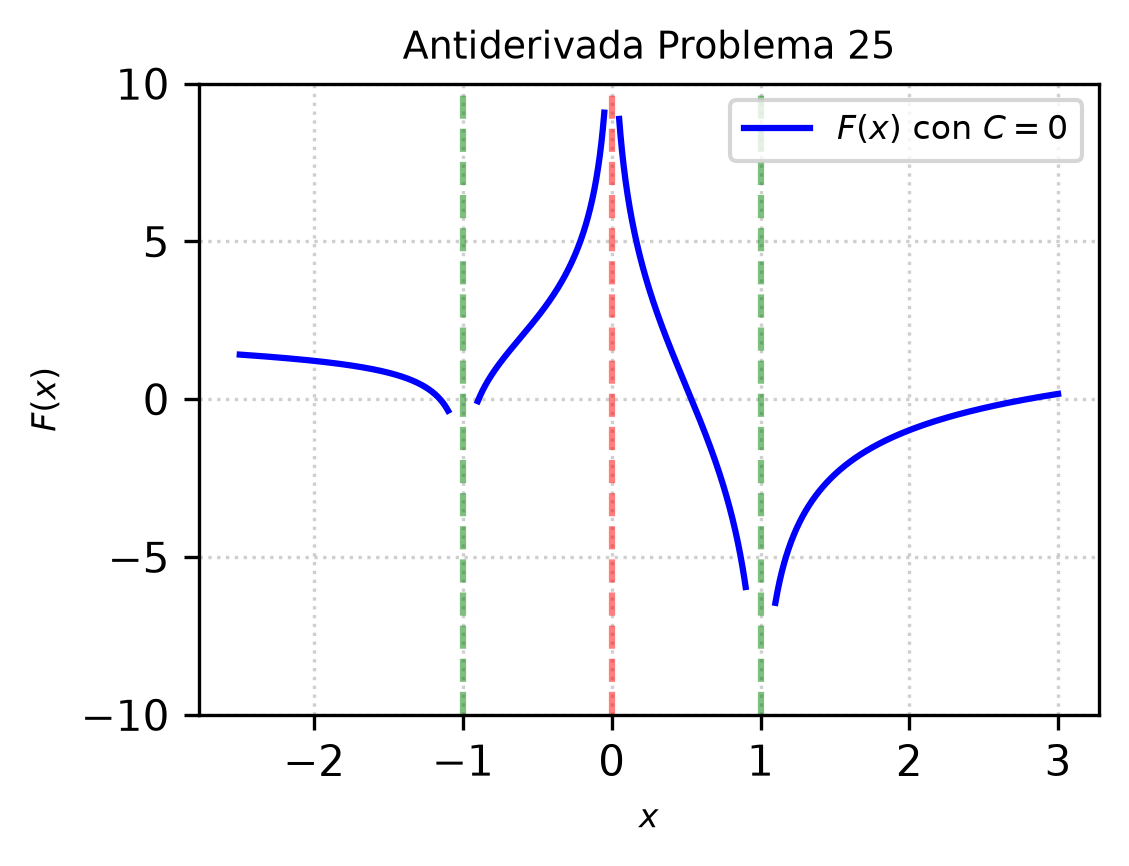
\includegraphics[width=\columnwidth]{semana_03/graficas/SEM03_P25_grafica.png}
	\caption{Representación gráfica de $f(x)$ y su antiderivada $F(x)$ evaluada para la constante de integración $C = 0$ (Problema 25).}
	\label{fig:problema25}
\end{figure}
